%\todo{ALETHIA - first draft by 30/May}

The search service provided by the Peer Manager (PM) was initially described in~\cite{D4.2}. In this deliverable we describe its evolution and provide more details about the meta-data models that are related with the search and ranking techniques, as well as their implementation.

\subsection{Mechanisms and algorithms}
%{\it including flow diagram, pseudo-code if needed, whatever explain how it works}

In order to select mechanisms and algorithms for implementing search in the PM we need to take into account existing approaches from the state of the art that can be used. For instance, there are many models and data structures that can be borrowed from the area of Information Retrieval (IR) as well as different matching techniques that can be used with different types of values. 

A logical view of the Search component is shown in Fig.~\ref{fig:search_diagram}, and presents the internal mechanisms, called subcomponents, that are integrated within the PM to deal with different types of queries (i.e., constraints on values of different natures). 
In what follows, these subcomponents are described in more details.

\begin{figure}[htbp]
\centering
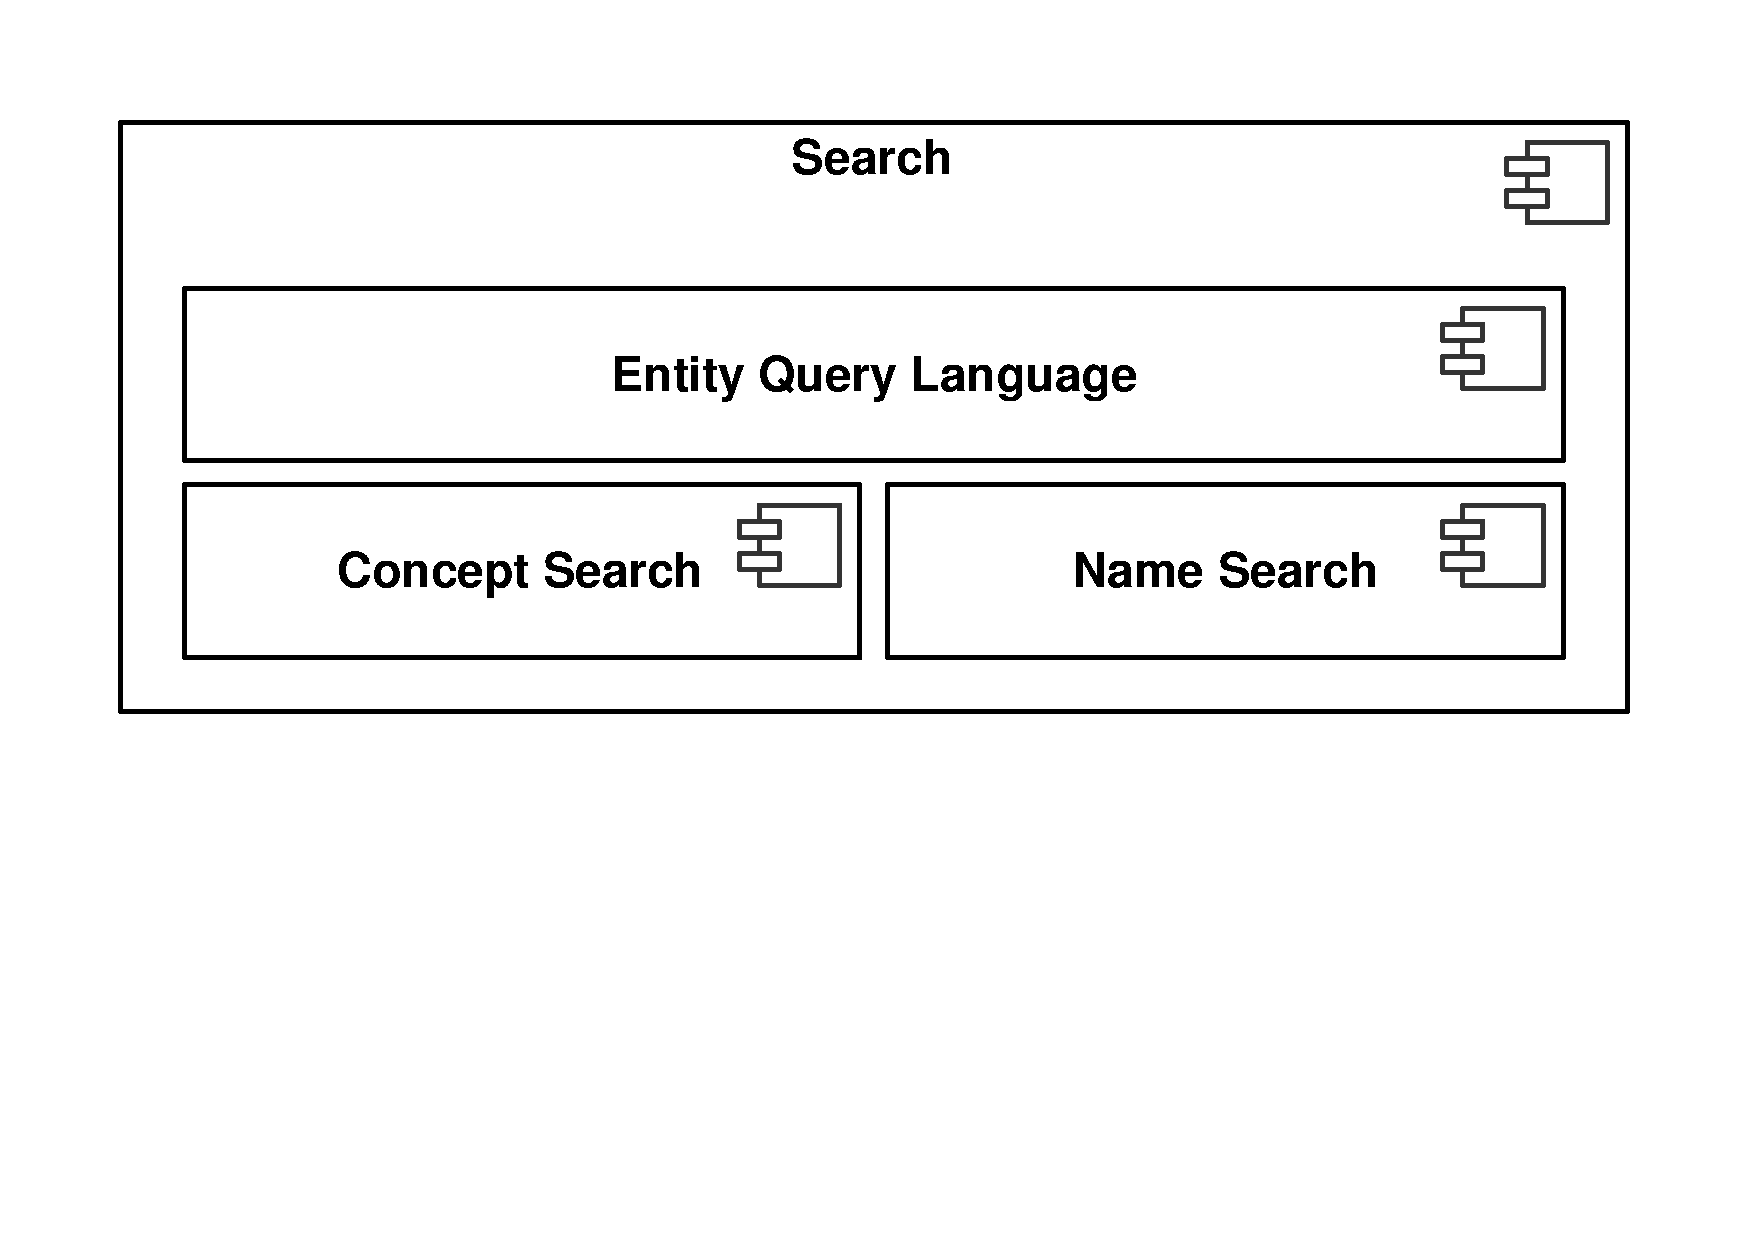
\includegraphics[width=0.65\textwidth]{figures/SearchComponentDiagram}
\caption{Search Diagram}
\label{fig:search_diagram}
\end{figure}

\paragraph{Concept Search.} 
\label{par:concept_search}
The lower part of Fig.~\ref{fig:search_diagram} shows two approaches that are used to deal with descriptions and names of peers. In particular, Concept Search, is used to match attributes from peers profiles with the search request. Concept Search~\cite{Giunchiglia:2009fk} was inspired by many syntactic IR systems that implement term matching by computing string similarity between words. For example, search for identical (possibly stemmed) words, words with common prefixes, words within a certain edit distance with a given word, or words that sound similar (see~\cite{Manning:2008:IIR:1394399} for more details on existing syntactic search approaches). 

However, when trying to match peer's attributes with a search query in the PM, there are many problems related with syntactic IR systems that can negatively affect the quality of search results. In particular, we know that different words can have the same meaning (synonymy); the same word may have multiple meanings (polysemy); and the meaning of words can be different but still semantically related. To deal with these problems, Concept Search extends the syntactic search approach with semantic search. In this approach, the retrieval models and data structures of syntactic search are reused. The main difference is given by the fact that concept search leverages on the core semantic data model of the PM and therefore concepts are used as terms instead of words. As a consequence, term matching is implemented by using semantic matching of concepts~\cite{Giunchiglia:2007ve}. On the other hand, when the semantic information is not available (i.e., when the concepts of a given set of words cannot be computed), words are used as terms and concept search falls back to the underlying syntactic search.


\paragraph{Name Search.} 
\label{par:name_search}
When dealing with peers that can be humans, it is important to account for the relevance of human readable identifiers (i.e., names). 
Names are labels composed by a combination of words, numbers and symbols. They are different from other attributes because they play the role of keywords rather than been mapped to concepts from a knowledge base. 
A name search algorithm deals with the problem of finding all the possible candidate entities that have names equal or similar to a given name.

Names can suffer from different types of variations, such as, format variations (e.g., \emph{George Augusto Lombardi} vs. \emph{George A. Lombardi} vs. \emph{Lombardi, George}), translations (e.g., \emph{Trento} in Italian vs. \emph{Trient} in German vs. \emph{Trent} in English), or misspellings (e.g., \emph{Fausot} vs. \emph{Fausto} vs. \emph{Fuasot}). These name variations show the complexity with which a name search algorithm has to deal. Various syntactic search techniques can be used for implementing name search. 

In the name search algorithm implemented by the PM, the following techniques are applied in a sequential order until the entities with the matching names are found:
\begin{inparaenum}[(i)]
\item \emph{Exact matching} between a given name and the entity name; 
\item \emph{Fuzzy search} techniques are employed by comparing name tokens using, for instance, jaccard~\cite{Bilenko:2003pd} similarity coefficient for comparing the similarity\footnote{\url{http://en.wikipedia.org/wiki/Similarity_measure}} of token sets.
\item Prefix search technique is used to perform fuzzy search on tokens themselves to account for the fact that, according to~\cite{Pollock:1984rr}, fewer errors usually occur at the beginning of names. 
%Search for name tokens having the same prefix can be efficiently implemented both in the inverted index vocabulary and by using SQL like queries.
\item Finally, the trigram search technique (N-gram index with grams of length 3) is used to account for the case of misspelled names. The pg\_trgm\footnote{\url{http://www.postgresql.org/docs/8.4/static/pgtrgm.html}}  module from PostgreSQL database management systems is used to implement trigram search on entity names in the current implementation. 
\end{inparaenum}


\paragraph{Entity Query Language.} 
\label{par:entity_query_language}
The upper part of the figure shows a subcomponent that builds on the two types of searches presented above and supports additional search operations based on the relations between entities. An Entity Query Language (EQL) provides more flexible and heterogeneous language to access peer’s attributes as well as additional operations. 
EQL is used by the PM to extend the low-level mechanisms. It can be seen as a semantically enabled version of HQL\footnote{\url{http://docs.jboss.org/hibernate/core/3.3/reference/en/html/queryhql.html}} on entities, where HQL is an object-oriented query language similar to SQL. More details about EQL are provided in the Annex~\ref{sec:search-annex}.


\subsection{Implementation}
%\todo{how it has been implemented} 

The Peer Manager's implementation of its search service (search, matching and ranking services) uses Java in combination with Hibernate and Spring frameworks, a PostgreSQL database is used for storage of peers' information and profiles. The Peer Manager front-end uses NodeJs and exposes its basic search functionalities through a low level HTTP API. In order to facilitate the interaction with other SmartSociety components (also in light of specific prototypes and demos), the PM provides also a high level API that results in more powerful and easy-to-use calls. Such calls leverage the full power of the Peer Manager and allow other components to abstract from internal details related to the PM's implementation. 

It is important to note that the implementation of the underlying mechanisms at the core of the PM's search implementation represent previous knowledge/work of the University of Trento Knowdive research group, so its source code will not be made commonly available. However, the full source code of the high level API corresponding to the front-end implementation that is specific for SmartSociety will be made available as part of the project. In the rest of this section we provide more details on how to use the search service, which in turn is related with the implementation of the high level API. 

\subsubsection{Search Service}\label{subsec:concept_search}
%\todo{documentation of search service including syntax/examples of EQL}

The Concept Search approach is used by the PM to implement concept based search on attributes from peers profiles.
The syntax of attribute-based concept search queries is designed to be similar to the query syntax of Lucene\footnote{\url{http://lucene.apache.org/core/old_versioned_docs/versions/3_5_0/queryparsersyntax.html}}, a popular Java based open-source indexing and search library. The current implementation supports concept search on attribute values, e.g. the query \emph{``big restaurant''} among other results will also return entities with attributes containing phrase \emph{``huge steakhouse''}. Concept search is also implemented on top of attribute names, e.g. the entity with attribute \emph{``location:Trento''} will be returned as an answer to query \emph{``place:Trento''}. Atomic queries on attribute values and attribute names can be combined into more complex queries by using Boolean operators, e.g. \emph{``big restaurant AND location:Trento''}.

The more flexible access to search services can be exploited through the specification of a search query using EQL language. The current implementation of the PM's search service supports only a subset of HQL, however, new features will be added if (and when) needed. The EQL implementation currently used in the PM supports the FROM clause, allowing the simplest query specification, as well as the SELECT, JOIN, GROUP BY, WHERE, and ORDER BY clauses that allow the specification of more complex queries. Among them, the ORDER BY clause is of key importance because is the one that is used to implement the ranking of search results. 

Note that concept search is used within FROM and SELECT clauses, which means that there is no need to know the exact name of the entity type or attribute name. Concept search approach is used for matching entity types in \emph{from} clauses and attribute names in \emph{select} clauses. 
 For instance, in the case when there is a synonymy relationship between concepts \emph{restaurant} and \emph{bar} in the underlying knowledge base, the search to find all the restaurants can also be performed by using the query ``\texttt{FROM bar r}''.
Another use of concept search query in \emph{from} clause can be to select a subset of all the entities for a given entity type. For instance, the query ``\texttt{FROM restaurant[description:steakhouse] r}'' requires that descriptions of found restaurant entities contain complex concepts which are more specific than complex concept for `steakhouse', e.g. `steakhouse in Trento'. \todo{Last sentence unclear, please clarify example}


%%%%%%%%%%%%%%%%%%%%%%%%%%
%%%%%%%%%%-Limitations-%%%%%%%%%%
%%%%%%%%%%%%%%%%%%%%%%%%%%

%On the other hand, the current limitations include:
%\begin{enumerate}
%\item \textbf{Joins:} Only inner join is supported, i.e., the keyword \emph{join} is used for specifying inner join.
%\item \textbf{Nulls:} If an attribute name is selected, then only NOT NULL attribute values will be returned.
%
%\begin{tabular}{ll}
%\texttt{SELECT cat FROM Cat cat} & [all cats will be found] \\
%\texttt{SELECT cat, cat.name FROM Cat cat} & [cats without names will be skipped] \\
%\end{tabular}
%\item \textbf{Aggregates:} Only simple aggregate functions on attributes are supported, e.g. count(cat).
%\item \textbf{Dots:} As in HQL, dot-notation is used for accessing entity attributes. There are limitations on how dots are used. The first (and only the first) dot defines an attribute (e.g. cat.name). The second dot can be used only for accessing the meta-data (e.g. cat.name.metadata). Note, that it is not really a limitation because all the queries with two or more dots can be rewritten by using explicit joins, as it is shown below:
%
%\begin{tabular}{p{0.45\textwidth}p{0.45\textwidth}}
%\texttt{SELECT cat.mate.name} & [not supported] \\
%\texttt{FROM Cat cat} & \\
% & \\
%\texttt{SELECT mate.name}  & [equivalent query with explicit join] \\
%\texttt{FROM Cat cat} & \\
%\texttt{JOIN cat.mate mate} & \\
%\end{tabular}
%\end{enumerate}


%%%%%%%%%%%%%%%%%%%%%%%%%%
%%%%%%%%%%-Additional notes-%%%%%%%
%%%%%%%%%%%%%%%%%%%%%%%%%%

%Additional notes:
%\begin{itemize}
%\item If no attribute is specified in select or where clause, entity id is used as a default attribute. For instance, 
%``\texttt{SELECT cat FROM Cat cat}'' internally, will be translated to ``\texttt{SELECT cat.id FROM Cat cat}''
%
%\item Specifying an alias (e.g. cat) is required. For instance, ``\texttt{FROM Cat cat}''
%
%\item If concepts with multi-words are used for defining types or attributes, spaces between words should be replaced with underscore `\_'. For instance, ``\texttt{SELECT cat.first\_name FROM Cat cat}''.
%
%\item Underscore `\_' can also be used for specifying correct concepts which should be used for attribute names and types. For instance, ``\texttt{SELECT cat.name\_123 FROM Cat\_321 cat}''.
%\end{itemize}
%


\subsubsection{Main Endpoints Documentation}
\todo{The specification of the search APIs with an example will be added here for the final version of this document.}

\begin{tabular}{llp{4cm}p{5cm}}
\toprule
Method & Api & Description & Example \\
\midrule
GET & /peers/search & Returns a set of profile of the peers that match with the characteristics specified in the input query & \\
\bottomrule
\end{tabular}











